\documentclass[a4paper]{article}    % define document layout
%\documentclass[draft]{article}     % use draft option in packages
%-----------------------------
% preamble
%-----------------------------
\usepackage[sumlimits,]{amsmath}    % math equations and formulas
\usepackage[utf8]{inputenc}         % use UTF-8 encoding
\usepackage[english]{babel}         % use English language
\usepackage{graphicx}               % insert images
%\usepackage[draft]{graphicx}        % do not render figures
\usepackage{subcaption}             % multiple images in one figure
\usepackage{hyperref}               % hyperlinks
\usepackage{float}                  % floating objects (figures, tables)
\usepackage{geometry}               % page size and margins
\geometry{a4paper, margin=1in}      % margins
\usepackage{ragged2e}               % text alignment
\usepackage[table]{xcolor}          % change cell color in tables
%\usepackage{multirow}               % merge rows in table

\graphicspath{                      % path for figures
    {../figures/} 
}

%-----------------------------
% body
%-----------------------------
\begin{document}

\begin{figure}
    \centering
    % UNICAMP logo
    \begin{subfigure}{0.45\textwidth}
        \centering
        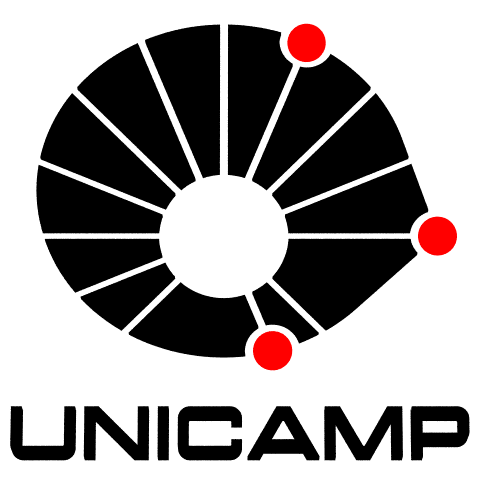
\includegraphics[width=1.5cm]{unicamp}
%        \label{fig:unicamp}
    \end{subfigure}
    \hfill
    % FEEC logo
    \begin{subfigure}{0.45\textwidth}
        \centering
        
\includegraphics[width=1.5cm]{feec}
%        \label{fig:feec}
    \end{subfigure}
\end{figure}

\title{
    \vspace{5cm}
    IA353A - Neural Networks\\
    EFC3
    \vspace{1cm}
}
\author{
    Rafael Claro Ito\\
    (R.A.: 118430)
    \vspace{11cm}
}
%R.A.: 118430
%ito.rafael@gmail.com
\date{July 2020}
\maketitle
\newpage

%=================================================
\section{Source files}
%=================================================

\paragraph{The Jupyter notebook with the code used to generate the plots and results presented in this report, all figures showed here and even the \LaTeX \space source code used to generate this PDF can be found at the following GitHub repository:}

\begin{center}
    {\url{https://github.com/ito-rafael/IA353A-NeuralNetworks-1s2020}}
\end{center}

%=================================================
\section{Q5 - Autoencoder}
%=================================================

%-------------------------------------------------
\subsection{1) Improving classes distribution}
%-------------------------------------------------

\href{https://colab.research.google.com/drive/1N7auSaSqYvORHTUK031ZfX4upoA38-hI?usp=sharing}{https://colab.research.google.com/drive/1N7auSaSqYvORHTUK031ZfX4upoA38-hI?usp=sharing}

%-------------------------------------------------
\subsection{2) CIFAR-10 DAE}
%-------------------------------------------------

\href{https://colab.research.google.com/drive/1v21h-yZRa7xRA1TcpUQR-H2eVin16VGy?usp=sharing}{https://colab.research.google.com/drive/1v21h-yZRa7xRA1TcpUQR-H2eVin16VGy?usp=sharing}

%=================================================
\section{Q6 - Time Series Forecasting}
%=================================================

%-------------------------------------------------
\subsection{P1 - NYSP}
%-------------------------------------------------

%------------------------
\subsubsection{Resumo geral}
%------------------------
Forneça o notebook devidamente executado, contendo, ao final, um resumo geral do que foi trabalhado em cada seção.

\href{https://drive.google.com/file/d/16gcoZosVIk0VwRFvws91Ul5WkAWhn0hT/view?usp=sharing}{https://drive.google.com/file/d/16gcoZosVIk0VwRFvws91Ul5WkAWhn0hT/view?usp=sharing}

%------------------------
\subsubsection{Preditor linear}
%------------------------
Com o foco no desempenho do preditor linear, procure apresentar argumentos capazes de sustentar o fato de a predição  proposta corresponder basicamente a uma versão atrasada da própria série temporal.

Analisando os pesos do preditor linear, podemos ver que o peso referente a entrada mais recente apresenta o maior peso dentre todos. Isso quer dizer que a última entrada vai ser a mais relevante para a predição do próximo passo. Isso faz com que a predição se assemelhe bastante ao valor imediatamente anterior, isto é, isso faz com que a predição seja semelhante a uma versão atrasada da série.

%------------------------
\subsubsection{Preditor não-linear}
%------------------------
Embora seja possível obter, com os modelos de predição não-lineares, um desempenho similar àquele do preditor linear (isso não é solicitado ao aluno, no entanto), explique por que o preditor linear é tão competente nesta tarefa de predição específica.

%------------------------
\subsubsection{Offset}
%------------------------
Procure justificar também por que alguns preditores não-lineares estão fornecendo uma predição que, aparentemente, falha apenas no offset da predição, ou seja, acompanham o comportamento da predição, mas erram no seu valor médio.

%-------------------------------------------------
\subsection{P2 - NLTS}
%-------------------------------------------------

%------------------------
\subsubsection{Resumo Geral}
%------------------------
Forneça o notebook devidamente executado, contendo, ao final, um resumo geral do que foi trabalhado em cada seção. Forneça, por exemplo, o número de atrasos da série temporal que está sendo considerado como entrada dos preditores e como está sendo feita a regularização dos modelos, quando for o caso.

\href{https://drive.google.com/file/d/1tfdgQF8e4sri5eUNZ5AqUNOX9_cRdBnG/view?usp=sharing}{https://drive.google.com/file/d/1tfdgQF8e4sri5eUNZ5AqUNOX9\_cRdBnG/view?usp=sharing}

%------------------------
\subsubsection{Preditor linear}
%------------------------
Dadas as características da série temporal, explique o motivo pelo qual o preditor linear saiu de primeiro colocado em desempenho, na Parte 1, para último colocado nesta Parte 2. 

%------------------------
\subsubsection{Preditor de múltiplos passos à frente}
%------------------------
Escolha um dos preditores e implemente a predição de múltiplos passos à frente (several time steps ahead), explicando como funciona a sua metodologia. 

%------------------------
\subsubsection{}
%------------------------
Sem a necessidade de implementações práticas, explique que modificações metodológicas você faria caso se constatasse que a série temporal é não-estacionária, mas com uma variação lenta de suas propriedades estatísticas ao longo do tempo.

%-------------------------------------------------
\subsubsection{P3 - Sunspot}
%-------------------------------------------------

\href{https://drive.google.com/file/d/1lC1S8KexCw_3wM_IMTYd2vussNTS1cDC/view?usp=sharing}{https://drive.google.com/file/d/1lC1S8KexCw\_3wM\_IMTYd2vussNTS1cDC/view?usp=sharing}

%=================================================
\section{Q7 - Interpretability}
%=================================================

\href{https://colab.research.google.com/drive/1qfos8-dzNBf2Wlg1XqOAoAL3KWB_hqgx?usp=sharing}{https://colab.research.google.com/drive/1qfos8-dzNBf2Wlg1XqOAoAL3KWB\_hqgx?usp=sharing}

%=================================================
\end{document}

